\chapter{Desenvolvimento embrionário dos vertebrados}\label{ch:b2:vertebrate-development}

O ovo de uma rã é uma esfera de dois milímetros de diâmetro, escura em
cima e clara embaixo. Em um dia, ele se dividiu em milhares de
células; em dois, uma lâmina dessas células se enrolou para dentro
através de um sulco para formar um intestino e depositar um bastão ao
longo do dorso; em três, a lâmina acima do bastão se dobrou num tubo
que será o encéfalo e a medula espinal. Nada foi acrescentado além de
água. A informação que transforma uma célula num girino nadador estava
no ovo e em seu genoma, e o modo como ela se desdobra --- \omterm{def:b2:vertebrate-development:egg}{clivagem},
gastrulação, neurulação, a \omterm{def:b2:vertebrate-development:induction}{indução} de cada parte por suas vizinhas ---
é reconhecivelmente o mesmo num peixe, numa galinha e num camundongo.
Este capítulo acompanha um embrião de vertebrado ao longo dessas
etapas e descreve os experimentos que mostraram como cada parte dele
recebe a informação do que deve se tornar.

\section{Do ovo à blástula}

\begin{definition}[O ovo e seus eixos]\label{def:b2:vertebrate-development:egg}
\index{polo animal}\index{polo vegetativo}\index{vitelo}\index{clivagem}
Um ovo de vertebrado já é polarizado antes da fecundação: o
\emph{polo animal} contém o núcleo e a maior parte do citoplasma; o
\emph{polo vegetativo}, o \emph{vitelo}, a reserva de proteínas e de
lipídios da qual o embrião viverá até se alimentar. A quantidade de
vitelo determina o padrão de tudo o que se segue: um ovo de ouriço-do-mar
ou de mamífero quase não tem vitelo e se cliva por inteiro em células
iguais; um ovo de rã tem uma quantidade moderada e se cliva por
inteiro, mas de modo desigual (células pequenas em cima, grandes
células ricas em vitelo embaixo); um ovo de peixe ou de ave é quase
todo vitelo e só se cliva num disco de citoplasma sobre ele. Na rã, o
ponto de entrada do espermatozoide fixa o segundo eixo: o córtex gira
trinta graus para longe dele, expondo um \emph{crescente cinzento} do
lado oposto ao ponto de entrada, e esse lado se tornará o dorso. A
\emph{clivagem} é uma série de mitoses rápidas sem crescimento --- as
células se reduzem à metade em cada uma ---, comandada por mRNAs e
proteínas maternos armazenados no ovo, enquanto os genes do próprio
embrião permanecem silenciosos até a \emph{transição da \omterm{def:b2:vertebrate-development:blastula}{blástula}
média}, após cerca de doze divisões.
\end{definition}

\begin{omfigure}
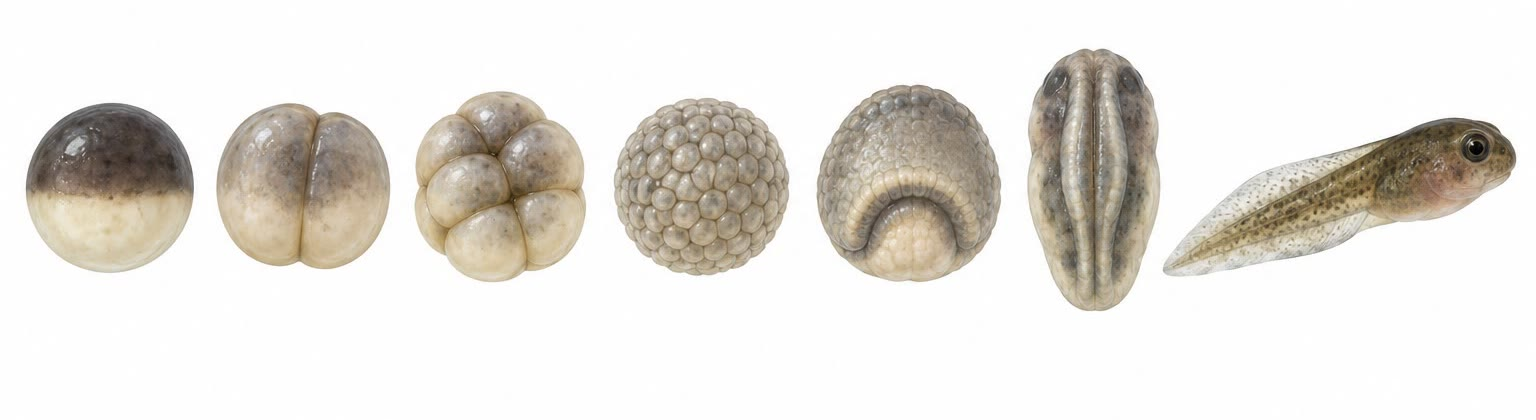
\includegraphics[width=0.9\linewidth]{images/book4/ai/b4-10-frog-development.jpg}

{\small O desenvolvimento de uma rã a partir do ovo fecundado: a
\omterm{def:b2:vertebrate-development:egg}{clivagem} até a \omterm{def:b2:vertebrate-development:blastula}{blástula}, a gastrulação, a nêurula com suas pregas
neurais e o girino --- tudo em poucos dias, sem crescimento.}
\end{omfigure}

\begin{theorem}[A aritmética da clivagem]\label{thm:b2:vertebrate-development:cleavage}
Após $k$ \omterm{def:b2:vertebrate-development:egg}{clivagens} síncronas, um ovo de volume $V_0$ é formado por
$2^{k}$ células de volume médio $V_0/2^{k}$ e raio $r_0/2^{k/3}$, e a
superfície total cresceu por um fator $2^{k/3}$; a razão entre o
volume nuclear e o citoplasmático, que começa perto de $10^{-4}$ num
ovo de rã, aumenta por um fator $2^{k}$ e atinge a de uma célula comum
($\sim 0.1$) após cerca de dez divisões. É essa razão crescente --- a
titulação de um estoque materno fixo de algum inibidor por uma
quantidade de DNA que cresce exponencialmente --- que desencadeia a
transição da \omterm{def:b2:vertebrate-development:blastula}{blástula} média: as divisões desaceleram, tornam-se
assíncronas e o genoma zigótico é ativado.
\end{theorem}
\begin{proof}
O volume se conserva na \omterm{def:b2:vertebrate-development:egg}{clivagem}, de modo que cada uma das $2^{k}$
células tem $V_0
2^{-k}$ e, como esfera, raio $r_0 2^{-k/3}$; sua área total é
$2^{k}\cdot 4\pi r_0^{2}\, 2^{-2k/3} = 4\pi r_0^{2}\, 2^{k/3}$. Cada
célula conserva um núcleo de tamanho fixo, de modo que a razão varia
como $2^{k}$ a partir de $10^{-4}$: $2^{10} = 1024$ a leva a $0.1$. A
transição da rã ocorre na décima segunda divisão, o que é coerente com
um limiar atingido um pouco mais tarde.
\end{proof}
\begin{proof}[Evidências]
Newport e Kirschner (1982) acrescentaram DNA extra a ovos de rã e
verificaram que a transição vinha mais cedo, tantas divisões quanto o
excesso de DNA; remover citoplasma tinha o mesmo efeito. O relógio não
é o tempo nem uma contagem de divisões, mas uma razão.
\end{proof}

\begin{definition}[Blástula]\label{def:b2:vertebrate-development:blastula}
\index{blástula}\index{blastocela}
A \omterm{def:b2:vertebrate-development:egg}{clivagem} termina numa \emph{blástula}: uma esfera oca (rã,
ouriço-do-mar) ou um disco (peixe, ave) de alguns milhares de células
em torno de uma cavidade, a \emph{blastocela}. Suas células ainda têm
aparência não especializada, mas não são equivalentes: um \emph{mapa de
destinos}, obtido corando manchas da superfície com corantes e
acompanhando-as, mostra que a calota animal dará a pele e o sistema
nervoso (\emph{ectoderma}), a faixa equatorial os músculos, o
esqueleto, o rim e o sangue (\emph{mesoderma}), e a massa vegetativa o
intestino e seus órgãos (\emph{endoderma}). Esses três \emph{folhetos
embrionários} são os mesmos em todos os vertebrados, e a etapa seguinte
é colocá-los em seus lugares: o mesoderma e o endoderma estão por fora
e precisam ir para dentro.
\end{definition}

\section{Gastrulação e neurulação}

\begin{proposition}[A gastrulação]\label{prop:b2:vertebrate-development:gastrulation}
\index{gastrulação}\index{blastóporo}\index{arquêntero}\index{notocorda}
A \emph{gastrulação} é o conjunto de movimentos celulares que
transforma a \omterm{def:b2:vertebrate-development:blastula}{blástula} de uma só camada numa \emph{gástrula} de três
camadas. Na rã, ela começa abaixo do crescente cinzento: as células ali
mudam de forma, contraindo suas extremidades externas em forma de
garrafa, e a superfície se dobra num sulco, o \emph{blastóporo}. Por
ele, o mesoderma e o endoderma fluem para dentro (\emph{involução}),
rolando sobre o lábio e avançando ao longo do teto da cavidade; a
calota animal se estende para baixo e recobre o exterior
(\emph{epibolia}); o blastóporo se fecha num anel em torno das últimas
células ricas em \omterm{def:b2:vertebrate-development:egg}{vitelo}. No interior, uma nova cavidade revestida de
endoderma, o \emph{arquêntero}, é o futuro intestino, e o mesoderma
que entrou primeiro, ao longo da linha média, tornou-se um bastão
rígido, a \emph{notocorda}, o eixo de todo embrião de vertebrado e a
estrutura que dá nome ao filo. Nas aves e nos mamíferos, os mesmos
movimentos ocorrem através de uma fenda, a \emph{linha primitiva}, num
disco achatado; nos peixes, o disco se espalha sobre o \omterm{def:b2:vertebrate-development:egg}{vitelo}. A
coreografia difere com o \omterm{def:b2:vertebrate-development:egg}{vitelo}; o resultado --- ectoderma por fora,
endoderma revestindo o intestino, mesoderma entre os dois, notocorda na
linha média --- é o mesmo.
\end{proposition}

\begin{omfigure}
\begin{tikzpicture}[every node/.style={font=\scriptsize}, >=stealth]
  % blastula
  \begin{scope}
    \draw[thick, fill=omDef!15] (0,0) circle (1.3);
    \draw[thick, fill=white] (0,0.2) circle (0.75);
    \fill[omExo!40] (0,0) ++(-1.3,0) arc (180:360:1.3 and 1.3) -- cycle;
    \draw[thick] (0,0) circle (1.3);
    \node at (0,0.2) {blastocela};
    \node[below, align=center] at (0,-1.45) {blástula\\calota animal (azul), células com vitelo (cinza)};
  \end{scope}
  % early gastrula: blastopore forming
  \begin{scope}[xshift=4.2cm]
    \draw[thick, fill=omDef!15] (0,0) circle (1.3);
    \draw[thick, fill=white] (0,0.25) circle (0.7);
    \fill[omExo!40] (0,0) ++(-1.3,0) arc (180:360:1.3 and 1.3) -- cycle;
    \draw[thick] (0,0) circle (1.3);
    \draw[very thick, omThm] (1.0,-0.85) .. controls (0.5,-0.6) and (0.4,-0.3) .. (0.55,0.0);
    \draw[->, thick, omThm] (1.15,-0.7) .. controls (0.6,-0.4) .. (0.4,0.1);
    \draw[omThm] (1.0,-0.85) -- (0.9,-1.25); \node[omThm, anchor=north west] at (0.6,-1.2) {lábio do blastóporo};
    \node[below, align=center] at (0,-1.45) {gástrula inicial\\as células rolam sobre o lábio};
  \end{scope}
  % late gastrula
  \begin{scope}[xshift=8.4cm]
    \draw[thick, fill=omDef!15] (0,0) circle (1.3);
    \draw[thick, fill=omExo!25] (0,0.05) circle (0.95);
    \draw[thick, fill=white] (0.15,-0.1) ellipse (0.55 and 0.4);
    \draw (0.6,-0.3) -- (1.6,-1.15); \node[anchor=west] at (1.6,-1.15) {arquêntero};
    \draw[very thick, omThm] (-0.9,0.35) .. controls (-0.2,0.6) .. (0.8,0.4);
    \draw[omThm] (0.0,0.48) -- (-0.9,1.55); \node[omThm, anchor=east] at (-0.9,1.55) {notocorda};
    \draw[thick] (1.1,-0.7) -- (1.3,-0.5);
    \node[right] at (1.3,-0.5) {blastóporo};
    \node[below, align=center] at (0,-1.45) {gástrula tardia: três camadas,\\cavidade intestinal, notocorda no teto};
  \end{scope}
\end{tikzpicture}

{\small A gastrulação na rã, em corte. As células rolam para dentro
sobre o lábio do blastóporo; o endoderma reveste uma nova cavidade
intestinal, e o primeiro mesoderma a entrar se torna a notocorda, ao
longo da linha média.}
\end{omfigure}

\begin{proposition}[A neurulação e o plano corporal]\label{prop:b2:vertebrate-development:neurulation}
\index{neurulação}\index{tubo neural}\index{somito}\index{crista neural}
O ectoderma acima da notocorda se espessa numa \emph{placa neural},
cujas bordas se elevam como pregas e se encontram na linha média,
formando o \emph{\omterm{prop:b2:vertebrate-development:neurulation}{tubo neural}}, futuro encéfalo e medula espinal, que
afunda sob a pele; células da crista das pregas, a \emph{\omterm{prop:b2:vertebrate-development:neurulation}{crista
neural}}, migram para formar os nervos periféricos, as células
pigmentares, a medula suprarrenal e grande parte da face. De cada lado
da notocorda, o mesoderma se segmenta em blocos, os \emph{somitos}, um
par após o outro, da cabeça à cauda, que dão as vértebras, os músculos
do tronco e a derme; o mesoderma lateral se divide nas camadas que
revestem a cavidade do corpo e formam o coração e os membros; o tubo
de endoderma forma por brotamento os pulmões, o fígado e o pâncreas. No
fim da neurulação, o embrião tem o plano corporal dos vertebrados ---
um cordão nervoso dorsal sobre uma notocorda, um intestino ventral,
musculatura segmentada, uma cabeça --- com um comprimento de poucos
milímetros, e o restante do desenvolvimento é a elaboração dos órgãos a
partir desse plano (\cref{ch:b2:limb-organogenesis}).
\end{proposition}

\begin{omfigure}
\begin{tikzpicture}[every node/.style={font=\scriptsize}]
  \foreach \x/\lab in {0/{placa neural}, 4.0/{as pregas neurais se elevam}, 8.0/{tubo neural fechado; a crista neural migra}} {
    \begin{scope}[xshift=\x cm]
      \draw[thick, fill=omExo!25] (-1.6,0) rectangle (1.6,-1.6);
      \draw[thick, omThm, fill=omThm!30] (0,-0.75) circle (0.28);
      \draw[thick, fill=omProp!30] (-1.3,-0.75) circle (0.32); \draw[thick, fill=omProp!30] (1.3,-0.75) circle (0.32);
      \node[below, align=center, text width=3.4cm] at (0,-1.7) {\lab};
    \end{scope}
  }
  \draw[very thick, omDef] (-1.6,0) -- (-0.7,0) .. controls (-0.3,0.15) and (0.3,0.15) .. (0.7,0) -- (1.6,0);
  \draw[very thick, omDef] (2.4,0) -- (3.3,0) .. controls (3.3,0.9) and (3.6,0.1) .. (4.0,0.0) .. controls (4.4,0.1) and (4.7,0.9) .. (4.7,0) -- (5.6,0);
  \draw[very thick, omDef] (6.4,0.05) -- (9.6,0.05);
  \draw[very thick, omDef, fill=omDef!20] (8.0,-0.3) circle (0.3);
  \foreach \p in {(7.35,-0.4),(8.65,-0.4)} \fill[omDef!70!black] \p circle (0.07);
  \node[omThm, anchor=west] at (9.8,-0.75) {notocorda};
  \node[omProp, anchor=west] at (9.8,-1.15) {somito};
  \node[omDef, anchor=west] at (9.8,-0.3) {tubo neural};
  \node[omDef!70!black, anchor=west] at (9.8,0.1) {células da crista neural};
\end{tikzpicture}

{\small A neurulação em corte transversal: o ectoderma sobre a
notocorda (vermelho) se espessa, se dobra e se fecha no \omterm{prop:b2:vertebrate-development:neurulation}{tubo neural}
(azul), enquanto o mesoderma ao lado da notocorda se segmenta em
somitos (laranja) e as células da \omterm{prop:b2:vertebrate-development:neurulation}{crista neural} deixam as pregas que
se fecham.}
\end{omfigure}

\begin{omfigure}
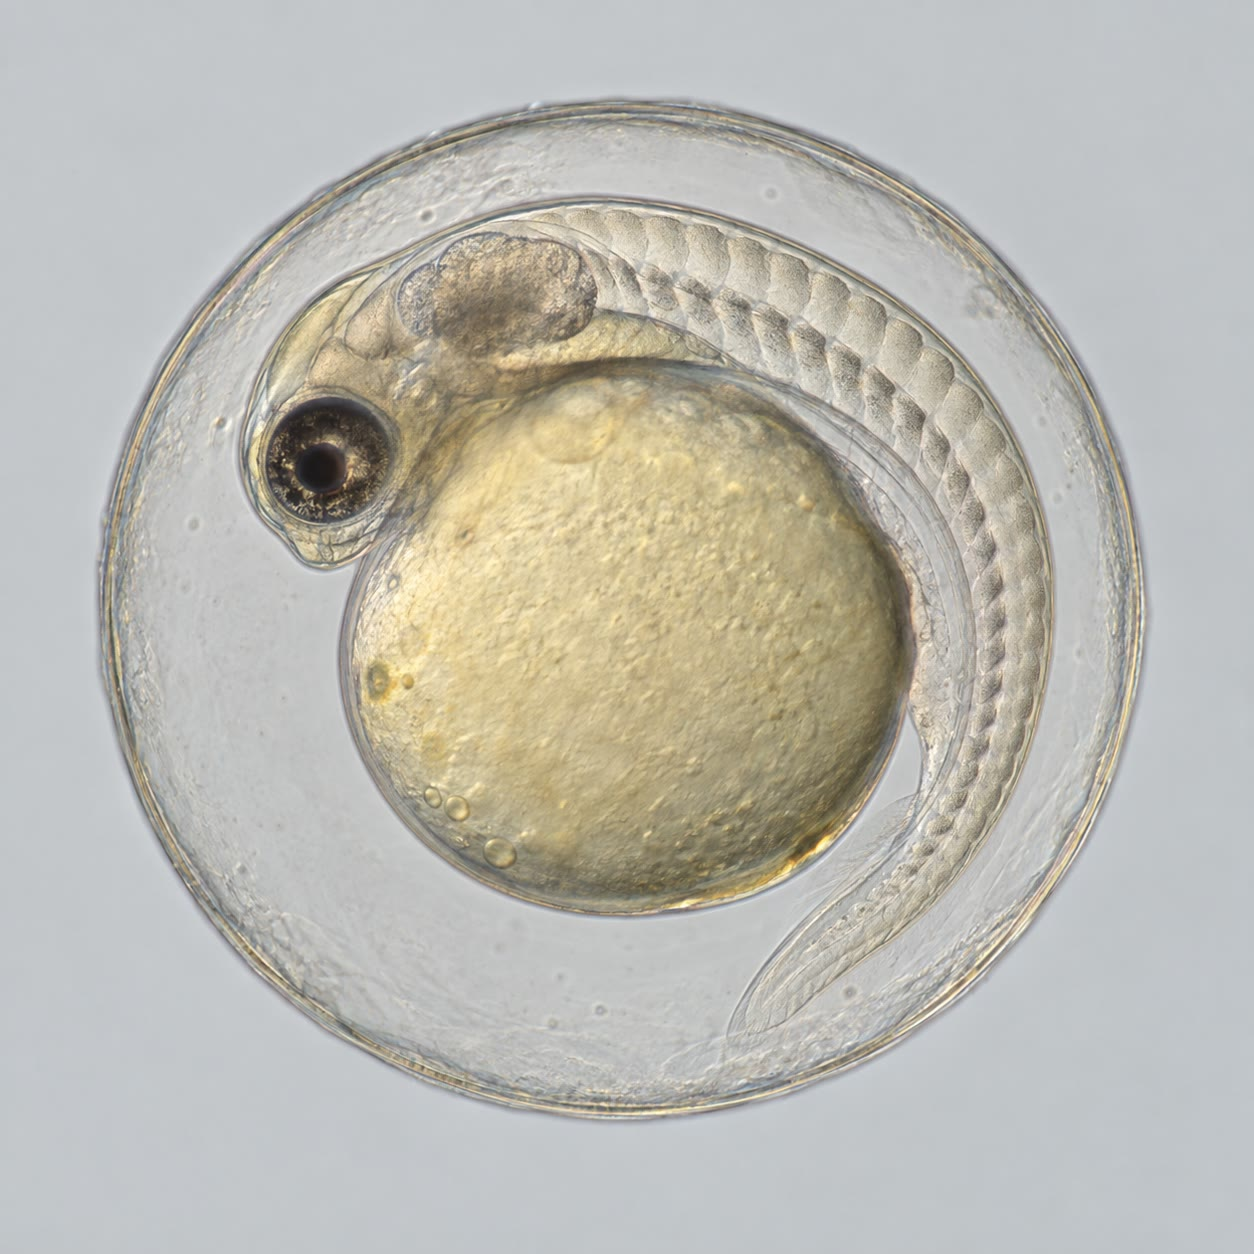
\includegraphics[width=0.42\linewidth]{images/book4/ai/b4-10-zebrafish-embryo.jpg}\hspace{0.04\linewidth}
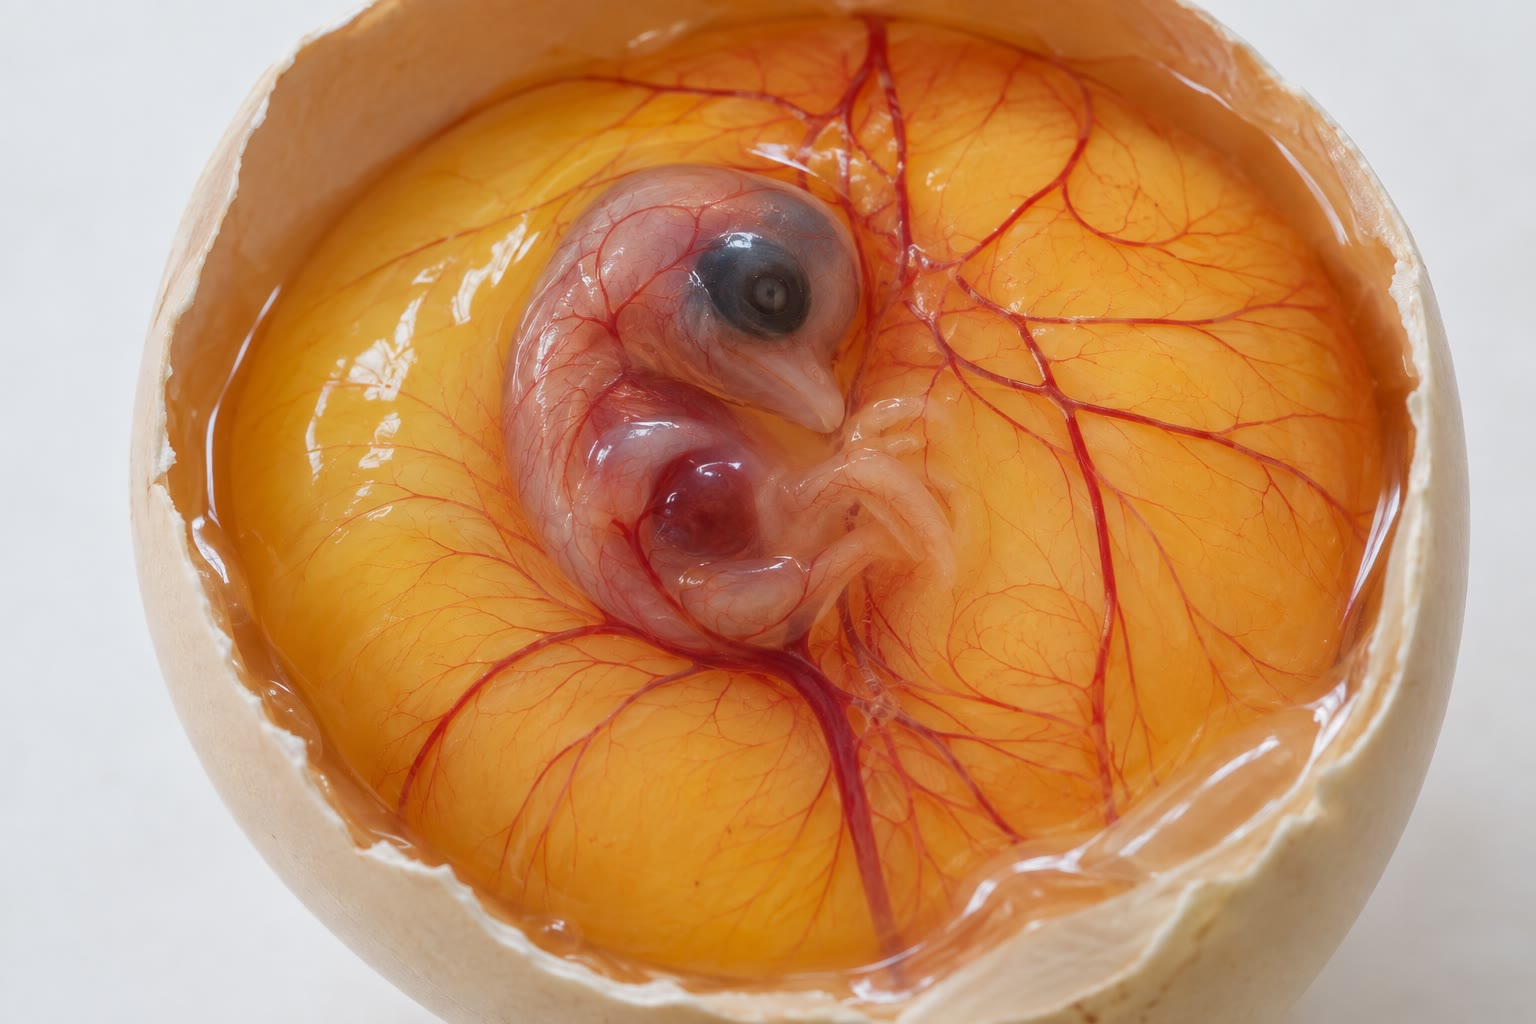
\includegraphics[width=0.5\linewidth]{images/book4/ai/b4-10-chick-embryo.jpg}

{\small À esquerda: um embrião de peixe-zebra de um dia dentro de seu
córion, enrolado em torno do \omterm{def:b2:vertebrate-development:egg}{vitelo}, com olho, encéfalo e uma fileira
de somitos. À direita: um embrião de galinha de três dias sobre seu
\omterm{def:b2:vertebrate-development:egg}{vitelo}, com o coração já batendo e os vasos se espalhando pelo \omterm{def:b2:vertebrate-development:egg}{vitelo}
para nutri-lo.}
\end{omfigure}

\section{Indução: como as células descobrem onde estão}

\begin{definition}[Indução e competência]\label{def:b2:vertebrate-development:induction}
\index{indução (embrionária)}\index{competência}\index{organizador}
A \emph{indução} é o processo pelo qual um grupo de células muda, por
meio de um sinal, o destino de um grupo vizinho; as células que
respondem precisam ser \emph{competentes} --- capazes de responder, o
que só são durante um tempo limitado. O desenvolvimento é uma cadeia de
induções: as células vegetativas induzem o mesoderma nas células acima
delas; o mesoderma dorsal --- o \emph{organizador}, no lábio do
blastóporo --- induz a placa neural no ectoderma acima dele e
padroniza o mesoderma de cada lado; a notocorda induz o assoalho do
\omterm{prop:b2:vertebrate-development:neurulation}{tubo neural}; a vesícula óptica, um broto do encéfalo, induz um
cristalino na pele que ela toca; o cristalino induz a córnea. Cada
tecido induzido se torna indutor do seguinte. Os sinais são um punhado
de famílias de proteínas secretadas, usadas repetidamente --- as mesmas
que padronizam um membro (\cref{ch:b2:limb-organogenesis}) e que, no adulto, comandam a
sinalização do \cref{ch:b2:cell-signalling}.
\end{definition}
\begin{proof}[Evidências]
Spemann e Mangold (1924) cortaram o lábio dorsal do blastóporo de uma
gástrula inicial de uma espécie de tritão e o enxertaram no lado
ventral de outra, de pigmentação diferente, para que as células do
hospedeiro e as do enxerto pudessem ser distinguidas. O enxerto não se
tornou simplesmente o que teria se tornado em seu lugar: ele rolou para
dentro, formou notocorda e \emph{induziu o próprio ectoderma ventral
do hospedeiro} a formar um segundo \omterm{prop:b2:vertebrate-development:neurulation}{tubo neural} e, ao lado dele,
somitos do hospedeiro --- um segundo embrião completo, em grande parte
feito de células do hospedeiro, unido ventre com ventre ao primeiro.
Nenhum outro pedaço da gástrula conseguia fazer isso. Eles chamaram o
lábio de \omterm{def:b2:vertebrate-development:induction}{organizador}; seus sinais (proteínas que bloqueiam o fator
ventralizante BMP) foram identificados setenta anos depois.
\end{proof}

\begin{omfigure}
\begin{tikzpicture}[every node/.style={font=\scriptsize}, >=stealth]
  % donor
  \draw[thick, fill=omDef!12] (0,0) circle (1.3); \node[above] at (0,1.4) {gástrula doadora (clara)};
  \draw[very thick, omThm] (0.85,-0.95) arc (-45:-20:1.3); \node[omThm, right] at (1.2,-0.8) {lábio dorsal};
  \draw[->, thick] (1.6,-0.3) -- (3.4,-0.3);
  % host
  \draw[thick, fill=omExo!45] (5,0) circle (1.3); \node[above] at (5,1.4) {gástrula hospedeira (escura)};
  \draw[very thick, omThm] (5.85,-0.95) arc (-45:-20:1.3); \node[omThm, right] at (6.2,-0.8) {lábio próprio};
  \draw[very thick, omThm] (4.15,0.95) arc (135:160:1.3); \node[omThm, left] at (3.9,1.0) {enxerto};
  \draw[->, thick] (6.6,-0.3) -- (8.4,-0.3);
  % result: twinned embryo
  \draw[thick, fill=omExo!45] (10.6,0) ellipse (1.8 and 1.1);
  \draw[very thick, omDef!70!black] (9.2,0.5) .. controls (10.0,0.8) and (11.2,0.8) .. (12.0,0.5);
  \draw[very thick, omDef!70!black] (9.2,-0.5) .. controls (10.0,-0.8) and (11.2,-0.8) .. (12.0,-0.5);
  \node[above] at (10.6,1.2) {resultado: dois eixos};
  \node[anchor=north, align=center, text width=4cm] at (10.6,-1.2) {um segundo tubo neural e somitos, feitos de células do \emph{hospedeiro}, induzidos pelo enxerto};
\end{tikzpicture}

{\small O experimento do \omterm{def:b2:vertebrate-development:induction}{organizador}. Um lábio dorsal enxertado no
ventre de outra gástrula induz as células do hospedeiro a formar um
segundo eixo embrionário.}
\end{omfigure}

\begin{theorem}[Um gradiente de morfógeno]\label{thm:b2:vertebrate-development:gradient}
\index{morfógeno}
Muitas \omterm{def:b2:vertebrate-development:induction}{induções} funcionam por meio de um \emph{morfógeno}: um sinal
secretado por uma fonte, que se espalha pelo tecido e é lido pelas
células segundo sua concentração local --- acima de um limiar, um
destino; acima de um limiar mais alto, outro. Um morfógeno produzido
por uma fonte plana à taxa $j$ por unidade de área, que se difunde com
coeficiente $D$ e é degradado à taxa $k$, tem em regime estacionário o
perfil exponencial
\[
c(x) = c_0\,e^{-x/\lambda}, \qquad \lambda = \sqrt{D/k}, \qquad c_0 = \frac{j}{\sqrt{Dk}},
\]
de modo que a distância a partir da qual a concentração cai abaixo de
um limiar $T$ é $x_T = \lambda\ln(c_0/T)$: um tecido pode ser
padronizado em faixas de largura fixa por limiares fixos. Com $D =
\qty{1e-12}{m^2/s}$ (uma proteína desacelerada pelas ligações que faz
ao se mover pelo tecido) e $k = \qty{1e-3}{s^{-1}}$ (uma meia-vida de
cerca de doze minutos), $\lambda = \sqrt{10^{-9}}\,\unit{m} \approx
\qty{32}{\micro m}$: alguns diâmetros celulares,
a escala na qual os campos embrionários são padronizados. Dobrar a
fonte dobra $c_0$ e desloca todas as fronteiras para fora em $\lambda
\ln 2$.
\end{theorem}
\begin{proof}
Em regime estacionário, a difusão equilibra a degradação:
$D\,c'' = k\,c$, cuja solução decrescente é $c = c_0 e^{-x/\lambda}$,
com $\lambda^2 =
D/k$. O fluxo que sai da fonte é $-Dc'(0) = Dc_0/\lambda = j$, o que
dá $c_0 = j\lambda/D = j/\sqrt{Dk}$. Fazendo $c(x_T) = T$, obtém-se
$x_T$; passar de $c_0$ a $2c_0$ acrescenta $\lambda\ln 2$ a esse valor.
\end{proof}

\begin{omfigure}
\begin{tikzpicture}
\begin{axis}[
  width=0.78\linewidth, height=5.6cm,
  axis x line=bottom, axis y line=left,
  xmin=0, xmax=120, ymin=0, ymax=1.1,
  xlabel={distância da fonte (\unit{\micro m})}, ylabel={morfógeno (relativo)},
  xlabel style={font=\small, at={(axis description cs:0.5,-0.13)}, anchor=north},
  ylabel style={font=\small},
  tick label style={font=\small}, xtick={0,32,64,96}, ytick={0,0.5,1},
  clip=false,
]
\fill[omThm!18] (axis cs:0,0) rectangle (axis cs:22,1.05); \node[font=\scriptsize, anchor=south] at (axis cs:11,1.05) {destino A};
\fill[omProp!18] (axis cs:22,0) rectangle (axis cs:61,1.05); \node[font=\scriptsize, anchor=south] at (axis cs:41,1.05) {destino B};
\fill[omExo!18] (axis cs:61,0) rectangle (axis cs:120,1.05); \node[font=\scriptsize, anchor=south] at (axis cs:90,1.05) {destino C};
\addplot[very thick, omDef, domain=0:120, samples=80] {exp(-x/32)};
\draw[dashed, gray] (axis cs:0,0.5) -- (axis cs:22,0.5) -- (axis cs:22,0);
\draw[dashed, gray] (axis cs:0,0.15) -- (axis cs:61,0.15) -- (axis cs:61,0);
\node[font=\scriptsize, anchor=west] at (axis cs:62,0.55) {limiar 1};
\node[font=\scriptsize, anchor=west] at (axis cs:62,0.2) {limiar 2};
\end{axis}
\end{tikzpicture}

{\small Um gradiente de morfógeno com $\lambda = \qty{32}{\micro m}$.
Dois limiares dividem o tecido em três faixas de destino celular, cujas
larguras são fixadas por $\lambda$ e pelas razões entre os limiares e a
concentração na fonte.}
\end{omfigure}

\begin{example}[A leitura do gradiente]\label{ex:b2:vertebrate-development:reading}
Na gástrula de rã, as células da zona marginal expostas a quantidades
graduadas de um sinal da família da ativina se tornam, da dose mais
alta à mais baixa, notocorda, músculo, rim e sangue; células
dissociadas da calota animal colocadas numa placa com uma dose limiar
mudam de destino dentro de um fator dois de concentração. No \omterm{prop:b2:vertebrate-development:neurulation}{tubo
neural}, um sinal da notocorda e da placa do assoalho se espalha para
cima e especifica, a partir de baixo, os neurônios motores e depois
classes sucessivas de interneurônios, em limiares separados por
poucos diâmetros celulares. As coordenadas do organismo estão escritas
em concentrações.
\end{example}

\section{Destino, comprometimento e o momento das decisões}

\begin{proposition}[Quando o destino de uma célula se fixa]\label{prop:b2:vertebrate-development:commitment}
\index{determinação}\index{regulação (embrionária)}
O \emph{destino} de uma célula é o que ela normalmente se tornará; sua
\emph{potência} é o que ela pode se tornar se for deslocada; ela está
\emph{determinada} quando seu destino já não muda com o ambiente. Os
embriões jovens \emph{regulam}: cada um dos dois primeiros blastômeros
de rã, separados, forma um girino pequeno e inteiro, e as primeiras
células de um embrião de mamífero são todas totipotentes --- é assim
que surgem os gêmeos idênticos. A determinação vem gradualmente e em
momentos diferentes para tecidos diferentes: um pedaço de ectoderma de
gástrula inicial enxertado no ventre se torna pele do ventre, e o mesmo
pedaço retirado de uma gástrula tardia forma uma placa neural onde quer
que seja colocado; no estágio de broto caudal, um campo de membro
transplantado para o flanco forma ali um membro. Na maioria dos
invertebrados, ao contrário, o destino é fixado cedo pelo citoplasma
que cada célula herda (desenvolvimento em \emph{mosaico}), e um
blastômero separado forma apenas a sua parte. A estratégia dos
vertebrados --- manter as células flexíveis e dizer-lhes o que fazer por
\omterm{def:b2:vertebrate-development:induction}{indução} --- é o que torna possíveis os gêmeos, a regeneração e o
experimento do \omterm{def:b2:vertebrate-development:induction}{organizador}.
\end{proposition}
\begin{proof}[Evidências]
Spemann (1901) amarrou um laço de cabelo em torno de um ovo de tritão
no estágio de duas células: se o laço ficava no plano do crescente
cinzento, de modo que cada metade recebesse uma parte dele, formavam-se
dois embriões completos; se ficava perpendicular, de modo que uma
metade tivesse todo o crescente, essa metade formava um embrião e a
outra, uma bola de tecido ventral. O crescente --- o futuro \omterm{def:b2:vertebrate-development:induction}{organizador}
--- era a única parte que não podia ser dividida.
\end{proof}

\begin{example}[O calendário de uma rã]\label{ex:b2:vertebrate-development:timetable}
A \qty{18}{\celsius}: fecundação; primeira \omterm{def:b2:vertebrate-development:egg}{clivagem} a \qty{1.5}{h},
depois a cada meia hora; \omterm{def:b2:vertebrate-development:blastula}{blástula} de \num{4000} células a \qty{7}{h};
transição da \omterm{def:b2:vertebrate-development:blastula}{blástula} média a \qty{8}{h}; gastrulação de \qty{10}{h} a
\qty{20}{h}; as pregas neurais se fecham a \qty{30}{h}; o coração bate a
\qty{2.5}{d}; eclosão e alimentação a \qty{4}{d}, como um girino de
\qty{6}{mm}. Um peixe-zebra faz o mesmo em um dia, uma galinha em três,
um camundongo em nove; um embrião humano gastrula na terceira semana e
fecha o \omterm{prop:b2:vertebrate-development:neurulation}{tubo neural} na quarta --- antes que a maioria das mulheres saiba
que está grávida, e é por isso que o folato, necessário ao fechamento
do \omterm{prop:b2:vertebrate-development:neurulation}{tubo neural}, é prescrito antes da concepção.
\end{example}

\section{Exercícios}

\begin{exercise}[$\star$]\label{exo:b2:vertebrate-development:1}
Defina \omterm{def:b2:vertebrate-development:egg}{clivagem}, \omterm{def:b2:vertebrate-development:blastula}{blástula}, gastrulação e neurulação, e cite a
estrutura que cada etapa produz.
\end{exercise}

\begin{exercise}[$\star$]\label{exo:b2:vertebrate-development:2}
Dê os três folhetos embrionários e, para cada um, quatro tecidos
adultos que dele derivam.
\end{exercise}

\begin{exercise}[$\star$]\label{exo:b2:vertebrate-development:3}
Como a quantidade de \omterm{def:b2:vertebrate-development:egg}{vitelo} modifica o padrão da \omterm{def:b2:vertebrate-development:egg}{clivagem} e da
gastrulação? Compare uma rã e uma galinha.
\end{exercise}

\begin{exercise}[$\star$]\label{exo:b2:vertebrate-development:4}
O que é a \omterm{def:b2:vertebrate-development:induction}{indução}? Dê três \omterm{def:b2:vertebrate-development:induction}{induções} na ordem em que ocorrem num
embrião de rã, indicando o indutor e o tecido que responde.
\end{exercise}

\begin{exercise}[$\star\star$]\label{exo:b2:vertebrate-development:5}
Um ovo de rã de raio \qty{1}{mm} se cliva doze vezes. Calcule o número
de células, seu raio médio e o fator pelo qual a superfície celular
total cresceu. Por que o embrião precisa da superfície adicional?
\end{exercise}

\begin{exercise}[$\star\star$]\label{exo:b2:vertebrate-development:6}
A razão núcleo/citoplasma começa em $10^{-4}$, e a transição da
\omterm{def:b2:vertebrate-development:blastula}{blástula} média ocorre quando ela atinge $0.4$. Após quantas divisões?
Se o ovo receber uma injeção de três vezes sua própria quantidade de
DNA, em que divisão a transição ocorre?
\end{exercise}

\begin{exercise}[$\star\star$]\label{exo:b2:vertebrate-development:7}
Um morfógeno tem $D = \qty{2e-12}{m^2/s}$ e uma meia-vida de
\qty{10}{min}. Calcule $k$ e $\lambda$. Dois limiares estão a
\qty{50}{\%} e \qty{10}{\%} da concentração na fonte: dê as larguras das
três faixas de destino.
\end{exercise}

\begin{exercise}[$\star\star$]\label{exo:b2:vertebrate-development:8}
No gradiente do exercício anterior, a fonte é dobrada por uma \omterm{def:b2:genome-diversification:mutation}{mutação}.
Quanto se desloca cada fronteira? E se, em vez disso, a taxa de
degradação dobrar?
\end{exercise}

\begin{exercise}[$\star\star$]\label{exo:b2:vertebrate-development:9}
Descreva o experimento de Spemann e Mangold, diga por que as duas
espécies precisavam diferir na pigmentação e diga o que o resultado
excluiu.
\end{exercise}

\begin{exercise}[$\star\star\star$]\label{exo:b2:vertebrate-development:10}
Preveja o resultado de: (a) um pedaço de futura placa neural de uma
gástrula inicial enxertado no ventre; (b) o mesmo pedaço retirado de
uma gástrula tardia; (c) um pedaço de ectoderma ventral colocado sobre
uma notocorda numa gástrula tardia; (d) a remoção de todo o \omterm{def:b2:vertebrate-development:induction}{organizador}
de uma gástrula inicial. Explique cada caso com as noções de
\omterm{def:b2:vertebrate-development:induction}{competência} e de determinação.
\end{exercise}

\begin{exercise}[$\star\star\star$]\label{exo:b2:vertebrate-development:11}
A primeira \omterm{def:b2:vertebrate-development:egg}{clivagem} da rã leva \qty{90}{min} e as onze seguintes,
\qty{30}{min} cada, a \qty{18}{\celsius}; a \qty{10}{\celsius}, cada
etapa é 2.5 vezes mais lenta. Em que momento a transição da \omterm{def:b2:vertebrate-development:blastula}{blástula}
média é atingida em cada temperatura? Explique por que a transição
ocorre com o mesmo número de células nas duas temperaturas, e o que
isso diz sobre o relógio.
\end{exercise}

\begin{exercise}[$\star\star\star$]\label{exo:b2:vertebrate-development:12}
``Um embrião de vertebrado é construído por diálogo; um de invertebrado,
por herança.'' Discuta o contraste entre o desenvolvimento regulativo e
o desenvolvimento em mosaico, suas consequências para os gêmeos e a
regeneração, e por que se trata de uma diferença de grau.
\end{exercise}

\section{Problema: Um embrião de rã cronometrado e padronizado}

\begin{problem}[{Problema de fim de semana --- um embrião de rã
acompanhado ao longo da clivagem, da transição da blástula média, da
gastrulação e da indução, com o gradiente de morfógeno calculado e os
enxertos clássicos previstos, até o número de células e o momento da
transição e as larguras das faixas de destino}]
\label{pb:b2:vertebrate-development:1}
Um ovo de rã tem raio de \qty{0.7}{mm} e um núcleo de raio
\qty{0.03}{mm} cujo conteúdo de DNA é $c$; cada \omterm{def:b2:vertebrate-development:egg}{clivagem} leva
\qty{30}{min}, após uma primeira de \qty{75}{min}. A transição da
\omterm{def:b2:vertebrate-development:blastula}{blástula} média ocorre quando o DNA total atinge $4000\,c$. Morfógeno:
$D =
\qty{1e-12}{m^2/s}$, meia-vida de \qty{20}{min}, concentração na fonte
$c_0$, limiares a $0.4\,c_0$ e $0.08\,c_0$.

\medskip
\noindent\textbf{Parte I --- A \omterm{def:b2:vertebrate-development:egg}{clivagem}.}
\begin{enumerate}
  \item Calcule o volume do ovo e o de seu núcleo, e a razão
        núcleo/citoplasma inicial.
  \item Após quantas \omterm{def:b2:vertebrate-development:egg}{clivagens} o DNA atinge $4000\,c$? Quantas células?
  \item Em que momento após a fecundação?
  \item Qual é então o raio celular médio, e a razão entre o volume
        nuclear e o volume celular se os núcleos conservarem seu
        tamanho? Comente.
  \item Por que fator a superfície celular total cresceu?
  \item Cada \omterm{def:b2:vertebrate-development:egg}{clivagem} exige a cópia do genoma: quanto DNA foi
        sintetizado no total, em unidades de $c$, e por que o embrião
        não precisa transcrever seus genes para isso?
  \item O que muda na transição, e que experimento mostra que ela é
        desencadeada por uma razão, e não por uma contagem?
\end{enumerate}

\medskip
\noindent\textbf{Parte II --- A gastrulação.}
\begin{enumerate}[resume]
  \item Onde se forma o blastóporo em relação ao ponto de entrada do
        espermatozoide, e o que fixou essa posição?
  \item Liste, em ordem, os tecidos que rolam para dentro através do
        blastóporo e suas posições depois disso.
  \item A gastrulação leva \qty{10}{h}, e a lâmina que sofre involução
        percorre \qty{2}{mm}. Calcule a velocidade celular média em
        micrômetros por minuto e compare com um fibroblasto rastejante
        (\qty{1}{\micro m/min}).
  \item Por que a gastrulação é impossível antes da transição da
        \omterm{def:b2:vertebrate-development:blastula}{blástula} média?
  \item Explique numa frase por que é a notocorda, e não o \omterm{prop:b2:vertebrate-development:neurulation}{tubo neural},
        a estrutura que define os cordados.
  \item Um fármaco que bloqueia a mudança de forma das células é
        aplicado no início da gastrulação. Preveja o embrião.
\end{enumerate}

\medskip
\noindent\textbf{Parte III --- O gradiente.}
\begin{enumerate}[resume]
  \item Calcule $k$ a partir da meia-vida, e $\lambda$.
  \item Calcule as posições dos dois limiares.
  \item Dê as larguras das três faixas de destino em micrômetros e em
        células de \qty{15}{\micro m}.
  \item A fonte é reduzida à metade. Recalcule as duas posições e diga
        qual faixa encolhe mais.
  \item Uma célula a \qty{60}{\micro m} da fonte é deslocada para
        \qty{10}{\micro m} antes de o gradiente ser lido; depois, após a
        leitura. O que ela se torna em cada caso, e por quê?
  \item Explique por que um perfil exponencial dá fronteiras cujas
        posições dependem do logaritmo da intensidade da fonte, e por
        que isso torna a padronização robusta.
\end{enumerate}

\medskip
\noindent\textbf{Parte IV --- Enxertos.}
\begin{enumerate}[resume]
  \item Preveja o resultado de enxertar um lábio dorsal no lado ventral
        de uma gástrula inicial, e de enxertar zona marginal ventral no
        lado dorsal.
  \item Preveja o resultado de enxertar um lábio dorsal no lado ventral
        de uma \emph{nêurula}, e explique a diferença.
  \item Um embrião de rã no estágio de duas células é separado ao longo
        do plano do crescente cinzento; outro, perpendicularmente a ele.
        Preveja os dois resultados.
  \item Uma calota animal é retirada de uma \omterm{def:b2:vertebrate-development:blastula}{blástula} e cultivada
        sozinha; a mesma calota é cultivada ao lado de células
        vegetativas. Preveja os tecidos formados.
  \item Por que o resultado de Spemann e Mangold exigia que hospedeiro e
        enxerto fossem distinguíveis, e o que teria mostrado um enxerto
        da espécie errada?
  \item Enuncie o resultado: o número da \omterm{def:b2:vertebrate-development:egg}{clivagem} e o momento da
        transição, o número de células e as larguras das três faixas.
\end{enumerate}
\end{problem}
